% !TeX encoding = UTF-8
%



\newpage



% Screencapturings von Knoten zum Nachbauen in bestimmten Testfällen.


\subsection{Testknoten}

Ein Bilderkatalog der die Knoten zeigt, deren Erstellbarkeit wir explizit prüfen. Hinweis: Mit Adobe Reader ab Version 9 ist es möglich den Knoten-Bau im PDF-Dokument als Animation abzuspielen.\\


	\subsubsection*{\glqq {"U}berleger\grqq}
	
	% TODO: Störende Vorschau umgehen.
		\begin{figure}[!h]
		
			\label{Abb:Test-Knoten:Ueberleger}
			\centering	
			
			\includemedia[activate=onclick]
			{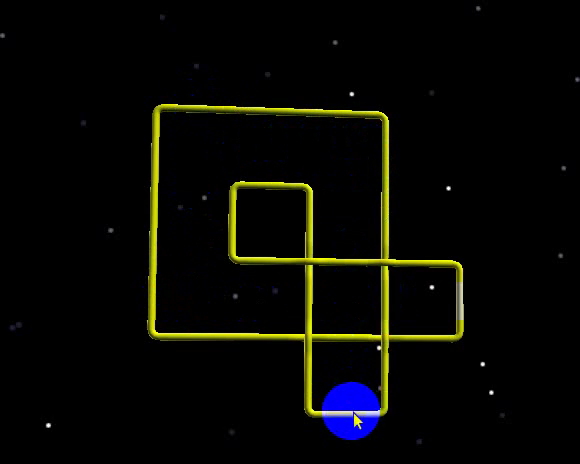
\includegraphics[width=\textwidth]
			{\KnotMedia/Ueberleger/Ueberleger.png}}
			{\KnotMedia/Ueberleger/Ueberleger.swf}
			
		\end{figure}
		
		~\\\mousecursor~\hyperref[FT:30:Ueberleger]{Zu Funktionstest FT\_30 (1.)} 
	
	

\clearpage	



	\subsubsection*{\glqq Schlaufe\grqq}	
	
		\begin{figure}[!h]
		
			\label{Abb:Test-Knoten:Schlaufe}
			\centering	
			
			\includemedia[activate=onclick %,
		%	width=1.0\textwidth,height=1.0\textwidth
			]
			{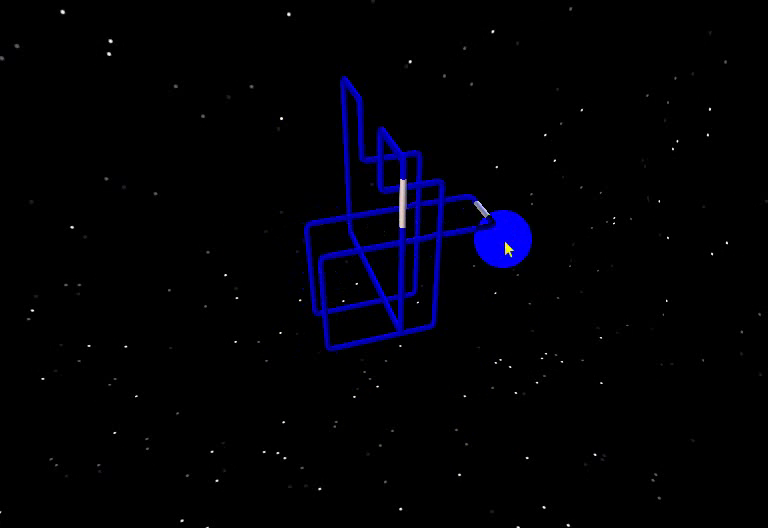
\includegraphics[width=\textwidth]
			{\KnotMedia/Schlaufe/Schlaufe.png}}
			{\KnotMedia/Schlaufe/Schlaufe.swf}
			
		\end{figure}
		
		~\\\mousecursor~\hyperref[FT:30:Schlaufe]{Zu Funktionstest FT\_30 (2.)} 
	
	

\clearpage	


